\chapter{Simulations}
\label{simulations}

In order to test and validate the different algorithms from chapter \ref{algos}, a simulation was implemented. The advantages of such simulations is to get rid of the technical compulsions of electronic materials, no configuration of the antennas was needed, no need to implement features in the application to deal with the \gls{cir}, no need to modify the state machines presented in appendix \ref{app:state_machine}, etc.
\vspace{2mm}

However, this simulation needs to be as true as possible compared with the reality. This implementation is detailed in the first section of this chapter. Then, the results obtained using this simulation are developed in the following sections for the locating methods in \ref{algos}.

\section{Simulation}

The simulation has been created by adapting a previously developed code for the project of the course of Communication Channel given at the ULB \cite{dedoncker2019course}. This simulation is based on the ray tracing, a technique used to compute the route of electro-magnetic waves detailed in section \ref{ray_tracing}. Two important features of this program can be separated. The first objective being to simulate a realistic \gls{cir} similar to the one produced by the experimental set-up. The second is to perform the localization based on this realistic \gls{cir}.
\vspace{2mm}

\subsection{Realistic CIR generation}

To reach this purpose, first the wished environment has to be simulated in the program. To make it happen, the $\texttt{room\_configuration.m}$ file has been created. Configuration of the geometry of the room, the type of walls used, the number of different furniture and their location in the room can also be chosen. This file is also used to choose the location of the anchor and the tag in the room. The left figure of the Fig. \ref{fig:peaks_real} has been produced using this configuration file.
\vspace{2mm}

In order to generate a finite-band \gls{cir}, the equivalent infinite-band \gls{cir} is first generated. This can be done for a direct ray, simple reflected ray, double reflected ray and triple reflected ray the transmission across the different materials is also taken into account. The ray reflected on the ground is also computed but not shown for the sake of clarity. An example of all the other ray can be found in Fig. \ref{fig:ray_simu}. On this figure, furniture are displayed against the walls, the direct ray is displayed in red, a simple reflected ray on one of the furniture in blue, a double reflected ray in cyan and a triple reflection ray is displayed in green.

\begin{figure}[H]
\centering
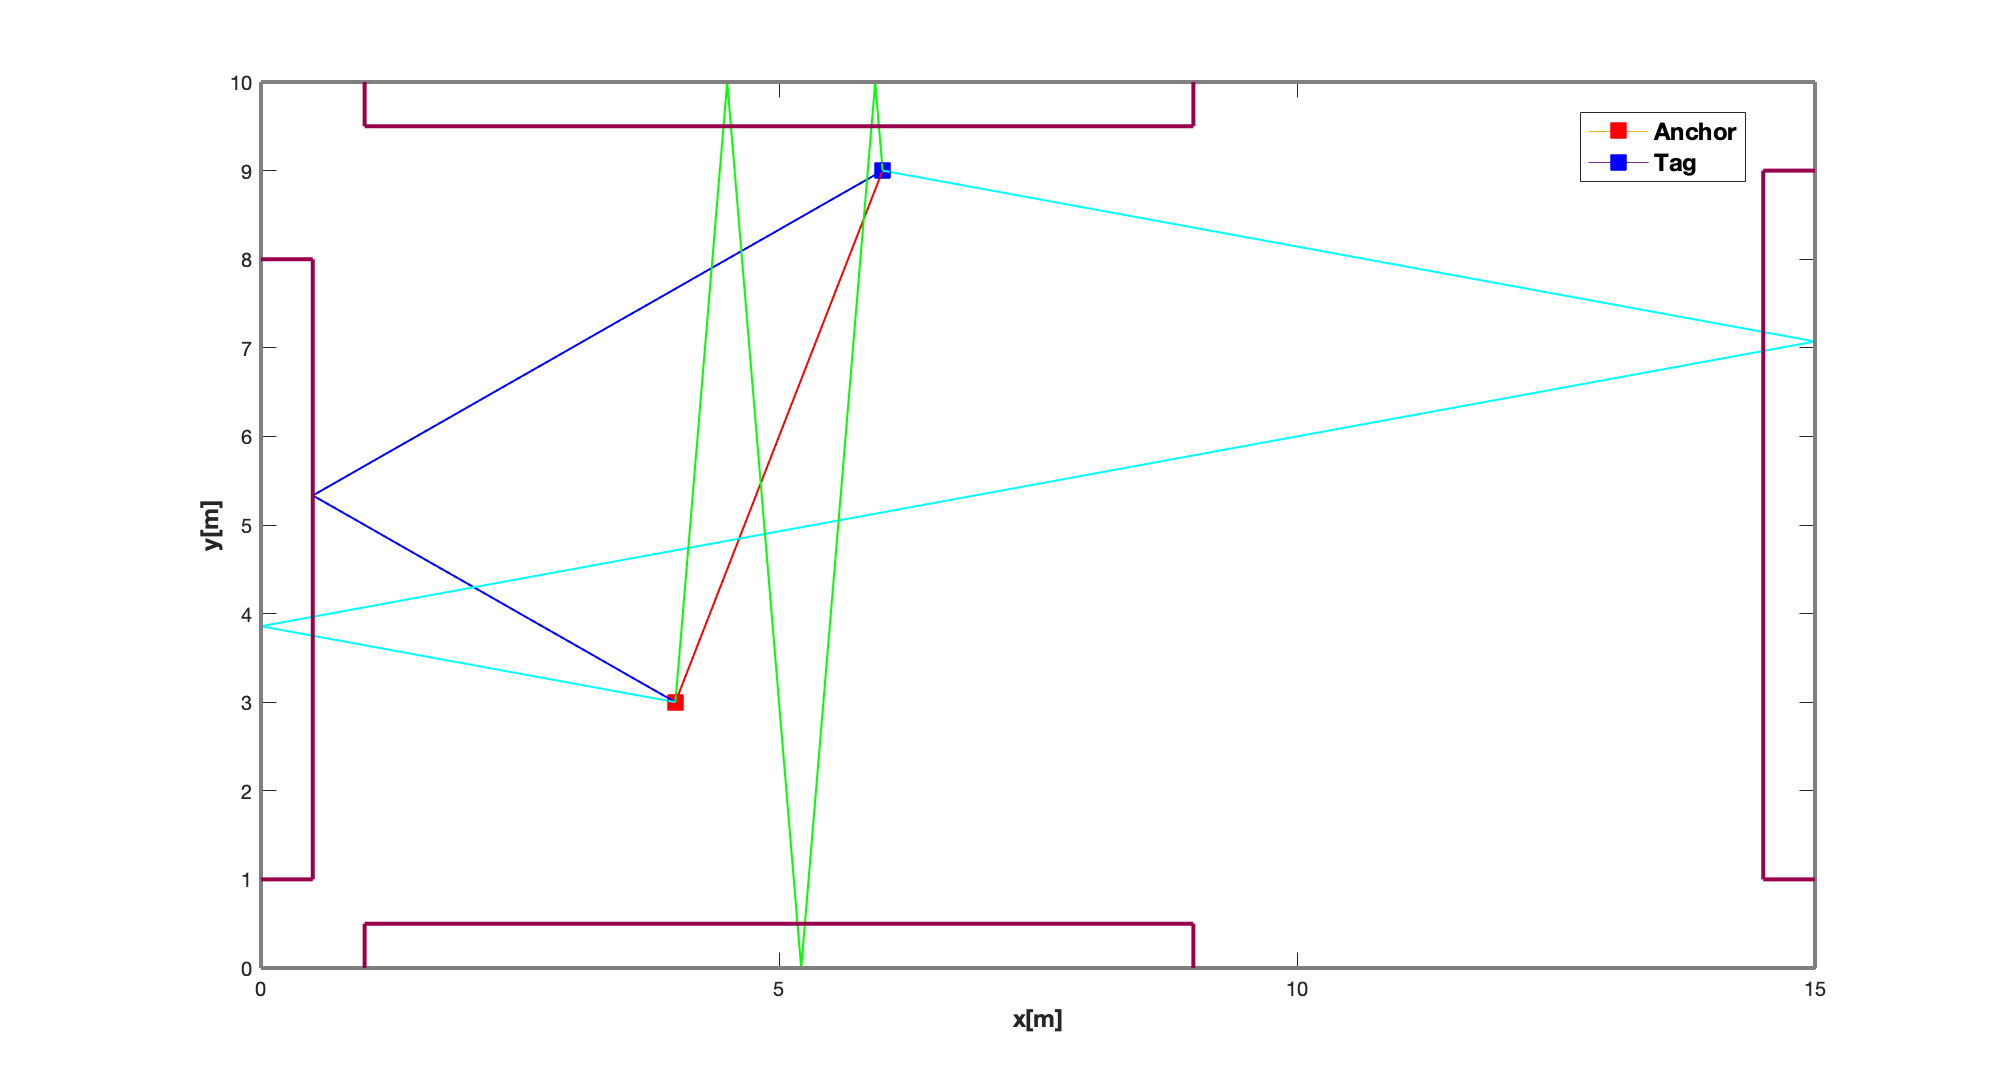
\includegraphics[width=.75\linewidth]{Images/rays_example.png}
\caption{Ray Tracing Simulation - Example. \label{fig:ray_simu}}
\end{figure}

Stating infinite is not completely correct, the real bandwidth being the one of the carrier frequency in this case, however, it shows the characteristics in connection with actual bandwidth used. The different peaks are well isolated and punctual. The so-called infinite-band \gls{cir} is converted to the frequency domain using the Fourier transform. The built-in \gls{fft} function from $\text{MATLAB}$ has been used \cite{mathworks}. The frequency spectrum has been reduced from the carrier frequency to $\text{500 MHz}$, an approximation of the bandwidth used as detailed in section \ref{dwm1000}. Using the \gls{ifft} to go back into the time domain results in the red curve on Fig. \ref{fig:conv_fin}.

\begin{figure}[H]
\centering
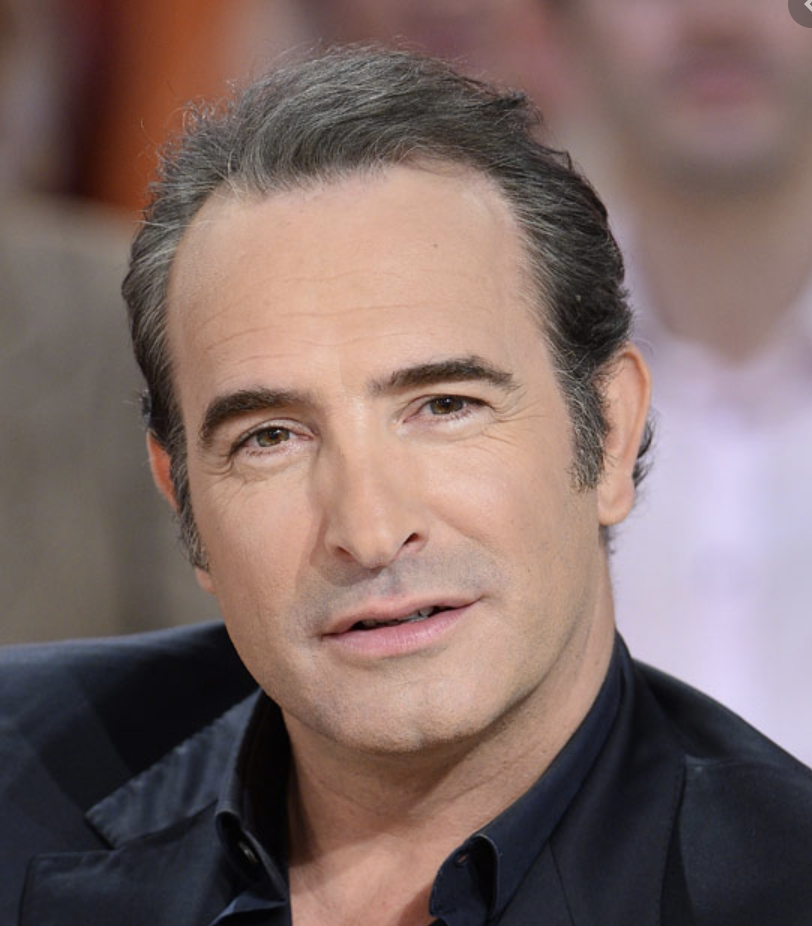
\includegraphics[width=.2\linewidth]{Images/Temporary_pic.png}
\caption{Trouver un nom \label{fig:conv_fin}}
\end{figure}

As we can observe, this \gls{cir} is far from ideal, mostly because of the sides lobes appearing next to every peak. This is a side effect due to the reduction of the bandwidth. In order to counter this effect, a Chebyshev window has been used \cite{lynch1997dolph}, \cite{mathworks}. The convolution of the finite-band time domain \gls{cir} will reduce those side lobes. The orange curve from Fig. \ref{fig:conv_fin} has been produced using a the $\text{chebyshev}$ function from MATLAB. The parameter of the Chebyshev window has been set heuristically to 25. A systematic method would have to use an experimental and a simulated \gls{cir} that would correspond to the same situation\footnote{The same room, antennas configuration, antennas position, ...}. The optimal parameter would then be computed using the $\text{lsqcurvefit}$ function from MATLAB.

\subsection{Code possible outputs ?}

The second objective of the simulation is the locating process. As detailed in the chapter \ref{algos}, two different method have been implemented in this scope. In order to compare both methods, \color{red}
to write \color{black}


\section{Soft Simulation}

\color{red}
Make an introduction
\color{black}

\gls{sla}.

\subsection{Symmetry issues}

An issue occurring with the 'one anchor' localization paradigm highlighted in section \ref{hard_loc} is the symmetry. This issue was discussed in the case of hard localization because of the axial symmetry between \glspl{va}, leading to mingled paths on the \gls{cir}. Another kind of symmetry issue can be seen on Fig. \ref{fig:square_sym}, approximatively half of the locations of the tag were correctly estimated.

\begin{figure}[H]
\centering
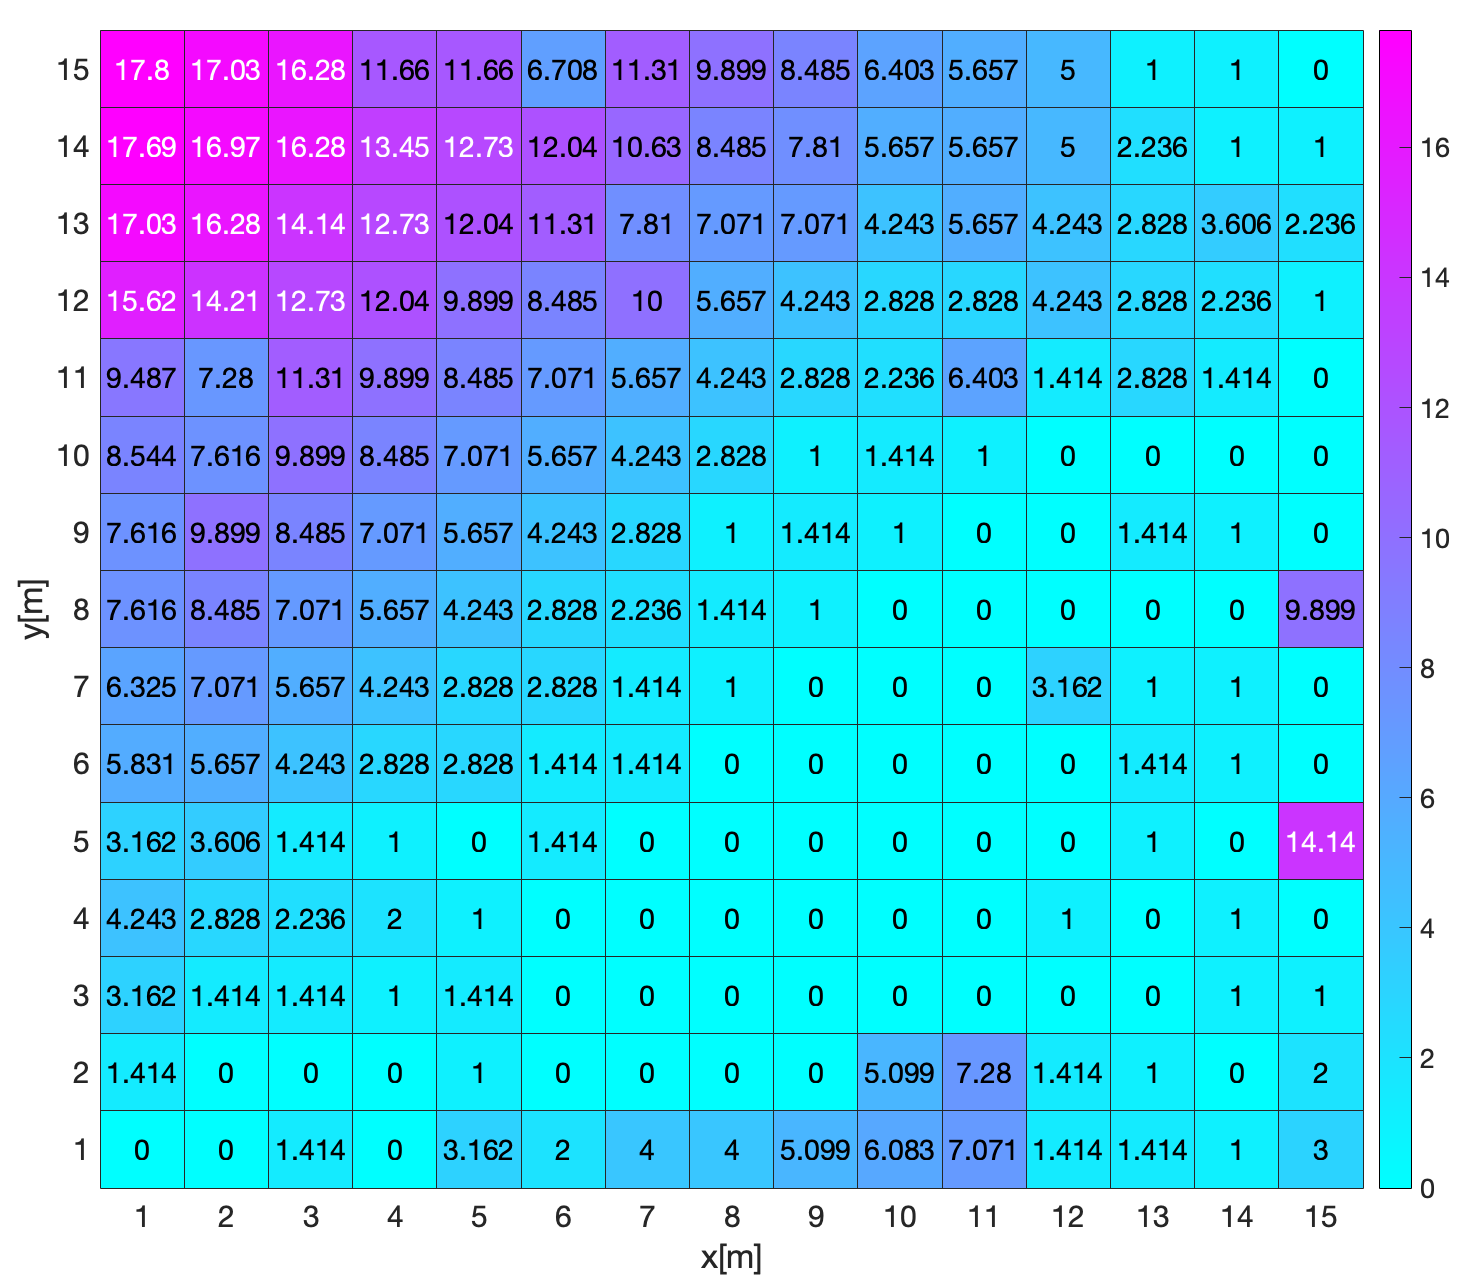
\includegraphics[width=.9\linewidth]{Images/15_15_sym.png}
\caption{Distance [m] between the tag exact location and the estimation provided by the \gls{sla}. Empty room of 15 by 15 meters, anchor set in (2, 2). Five peaks extracted from the CIR. \label{fig:square_sym}}
\end{figure}

Because of the location of the anchor, a symmetry appears in this room, the axial symmetry being the diagonal starting at the bottom left until the top right of the Fig. \ref{fig:square_sym}. This is confirmed by Fig. \ref{fig:square_sym_cir_comparison}. The \gls{mse} for each possible location in the solution space generated by the space solution reduction algorithm is shown. One can observe the symmetry across the bottom-left to top-right diagonal. This symmetry is not completely perfect, some location gets a small location error as (5, 2), which wrongly estimate the location by 1 meter, the origin of such particular cases is studied section \ref{soft_empty_room}.

\begin{figure}[H]
\centering
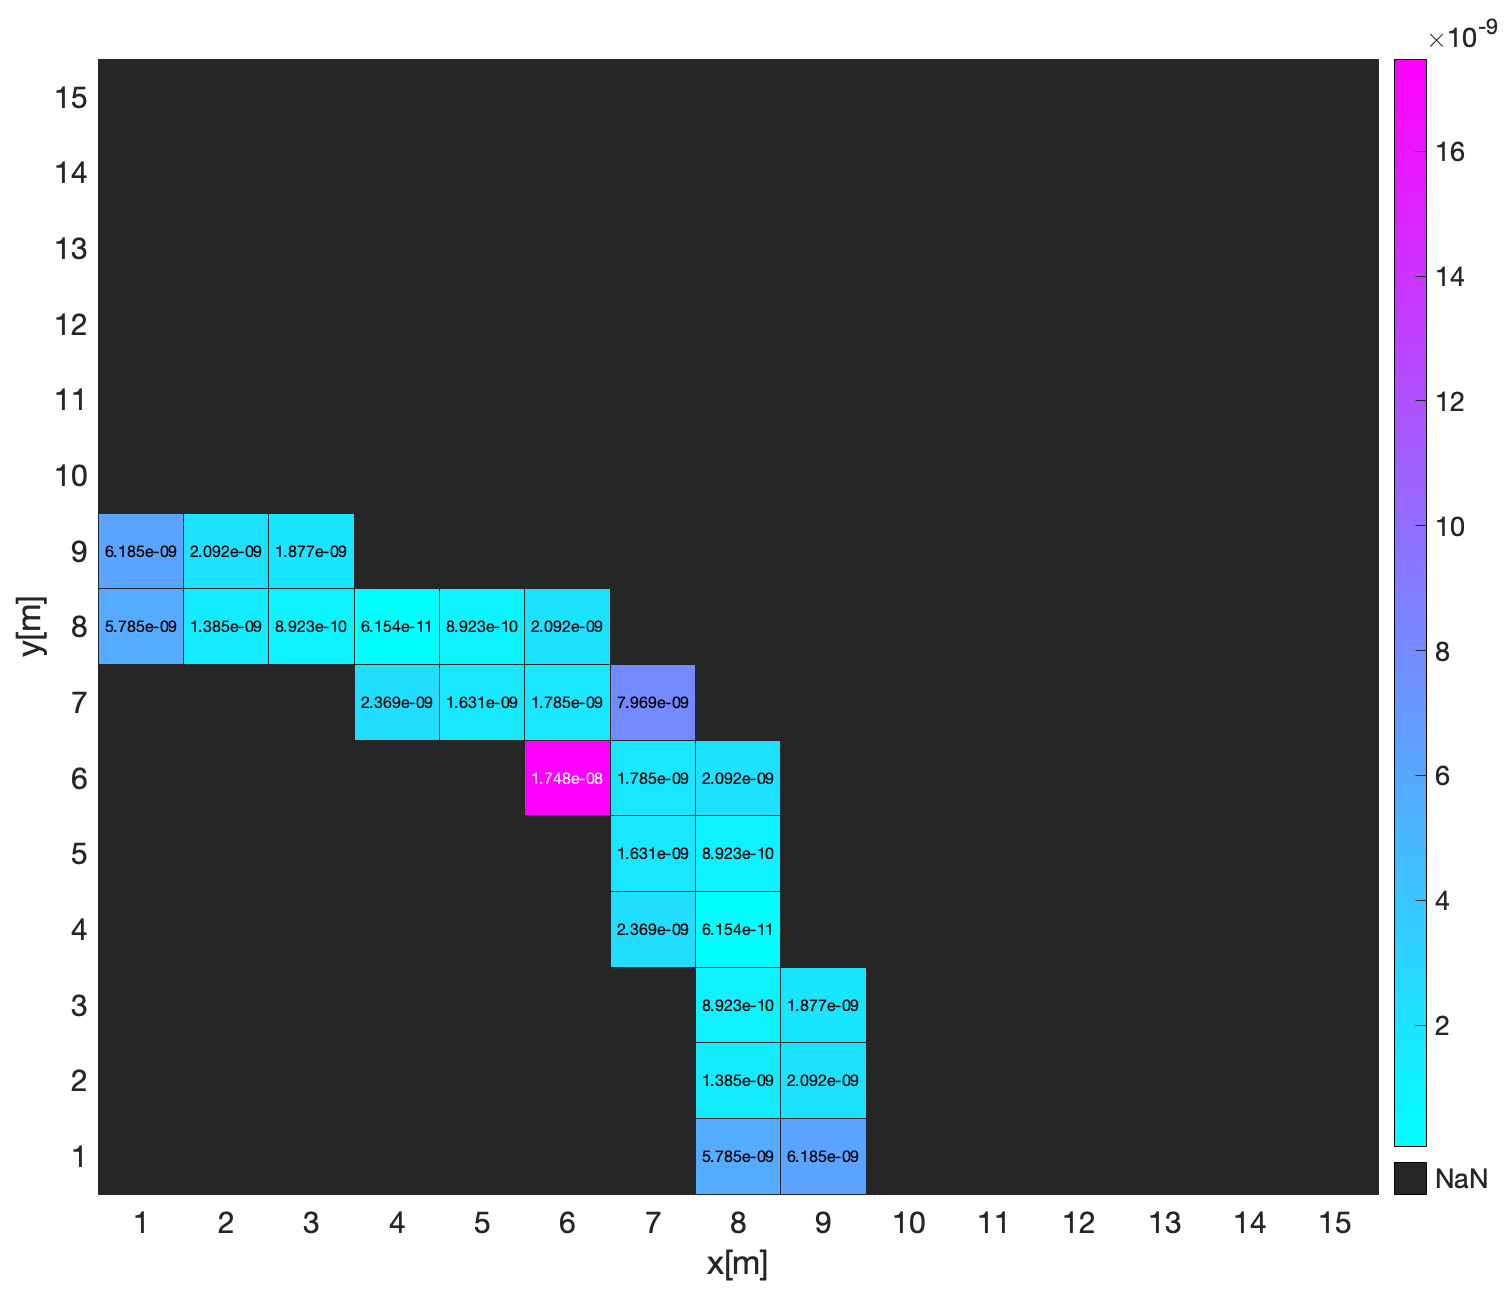
\includegraphics[width=.9\linewidth]{Images/square_sym_mse_4_8.png}
\caption{MSE between BLABLABLA \label{fig:square_sym_cir_comparison}}
\end{figure} 

To avoid such error, we should avoid placing the anchor in a such symmetric position. We can even generalize this result by stating that we should avoid to set the anchor on any axis of symmetry of the room, being the diagonals and the medians in a square. Such cases are shown in appendix \ref{app:symmetry_antenna_placement}, where the anchor has been set on a axis of symmetry.
\vspace{2mm}

We could assume that this issue only occurs in square rooms and not in rectangular rooms. Indeed, the diagonals of a rectangle are not part of its axis of symmetry, only its medians are. If those anchor are not on an axis of symmetry, there is no reason to obtain systematically twice the same \gls{cir}. Therefore, we could think that by avoiding those axis, this symmetry issue would also be avoided.
\vspace{2mm}

However, as it is shown on Fig. \ref{fig:rect_sym}, part of the \gls{cir} generated for (3, 7) and (7, 3) are the same when the anchor is set at (2, 2). The three extracted peaks, corresponding to the direct ray and the once reflected rays on the bottom and left walls, are equivalent, the beginning of the \gls{cir} being mostly identical in the two cases. We can conclude that the number of peaks extracted is an important parameter of this locating system. If too few peaks are taken, it may be impossible to distinguish several cases. If too many are taken, some irrelevant peaks could be extracted from the realistic \gls{cir}. This one being noisier because of the different reflections happening.

\begin{figure}[H]
\centering
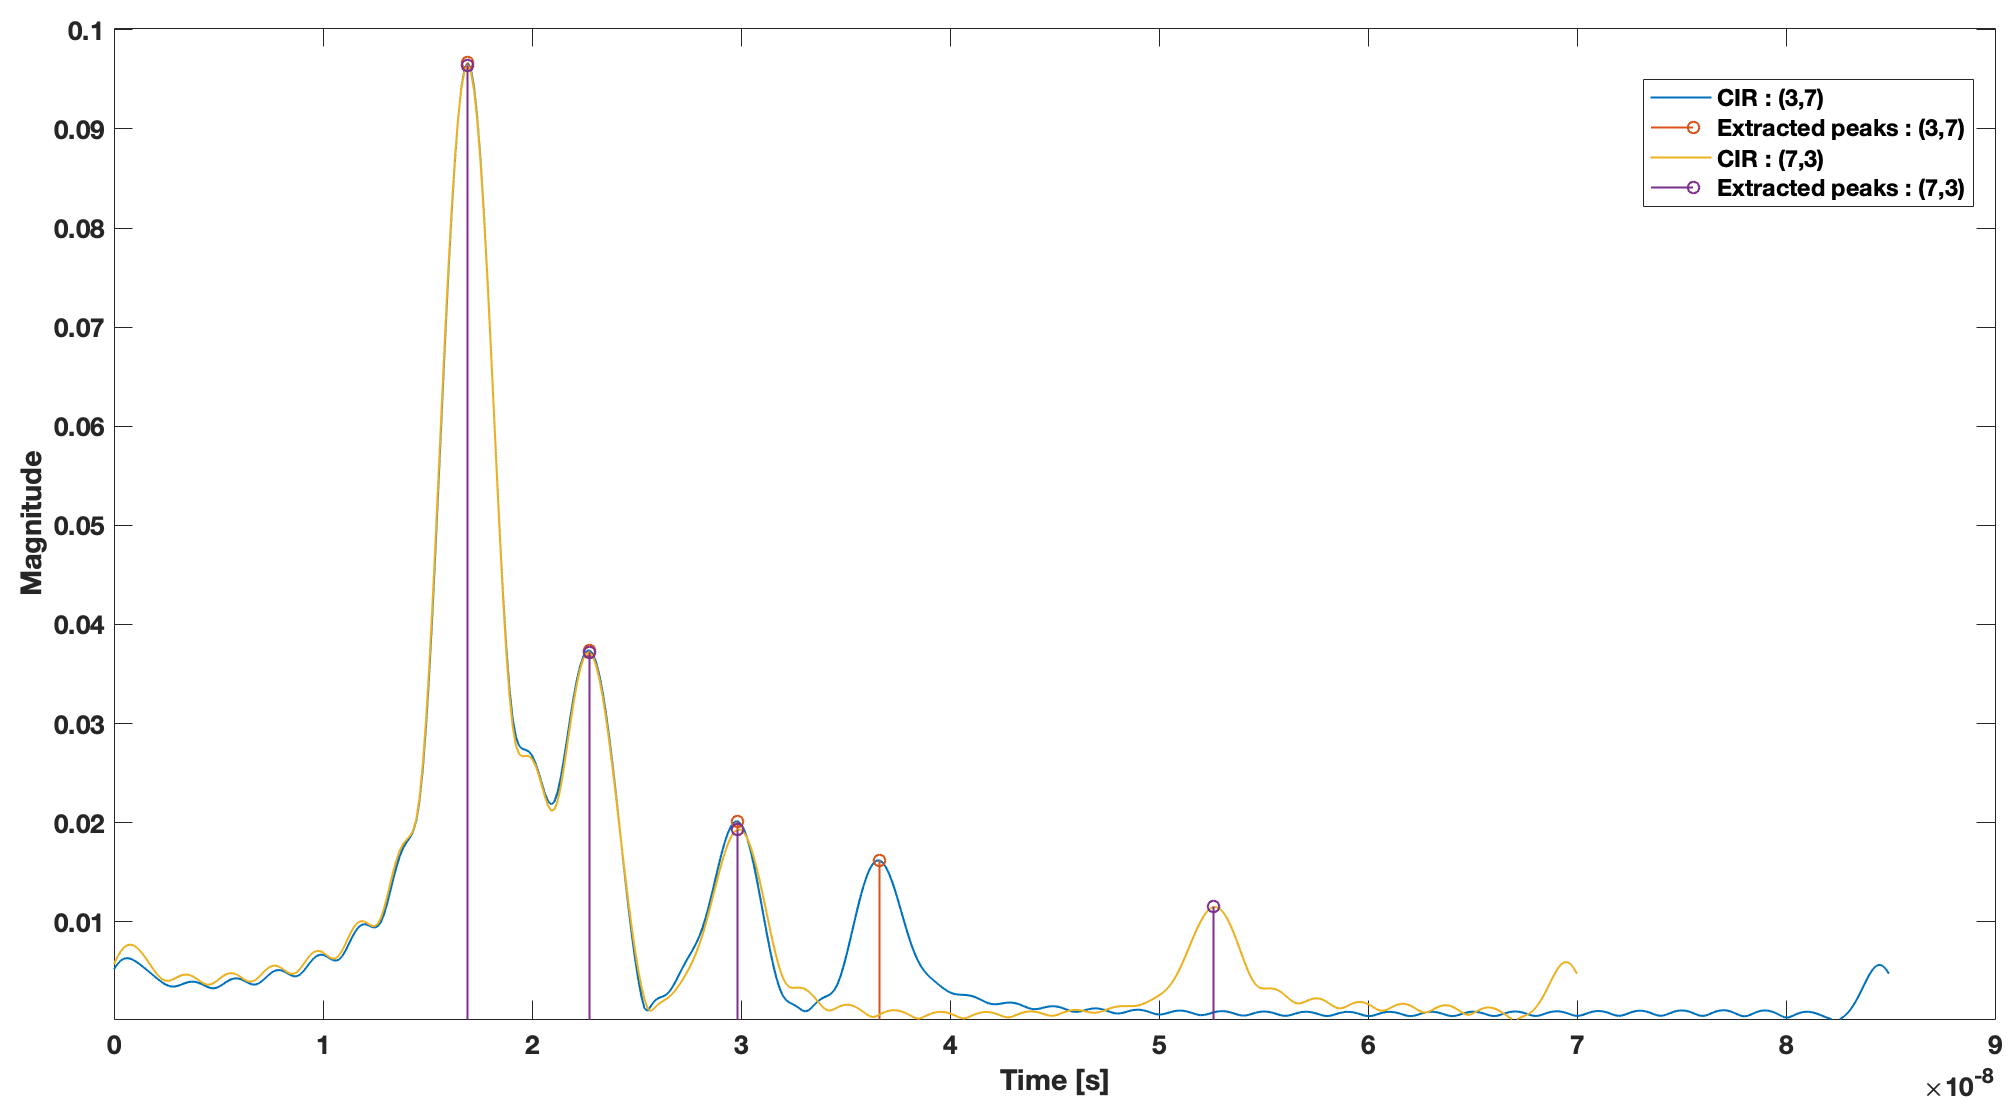
\includegraphics[width=.8\linewidth]{Images/cir_comparison_rect.png}
\caption{Comparison between two CIR obtained in a rectangular room (10 by 15)m. The anchor being located in (2, 2). \label{fig:rect_sym}}
\end{figure}

\subsection{Soft localization in an empty room}
\label{soft_empty_room}
Fig. \ref{fig:pos_ant_empty_non_sym} represents a room of dimension 10 by 15 m, with an anchor which is not set on any axis of symmetry. The chosen location of the anchor, which is (3, 1), is arbitrary and has mostly been chosen to avoid any location suffering from the symmetry. As we can observe, more than half of the location were correctly recovered and more than two third were almost correctly recovered\footnote{Exactly 86 over 150 were correctly recovered and 115 over 150 were almost correctly recovered. Almost meaning that the max distance between the tag and its location estimation is at most 1.5m.}.

\begin{figure}[H]
\centering
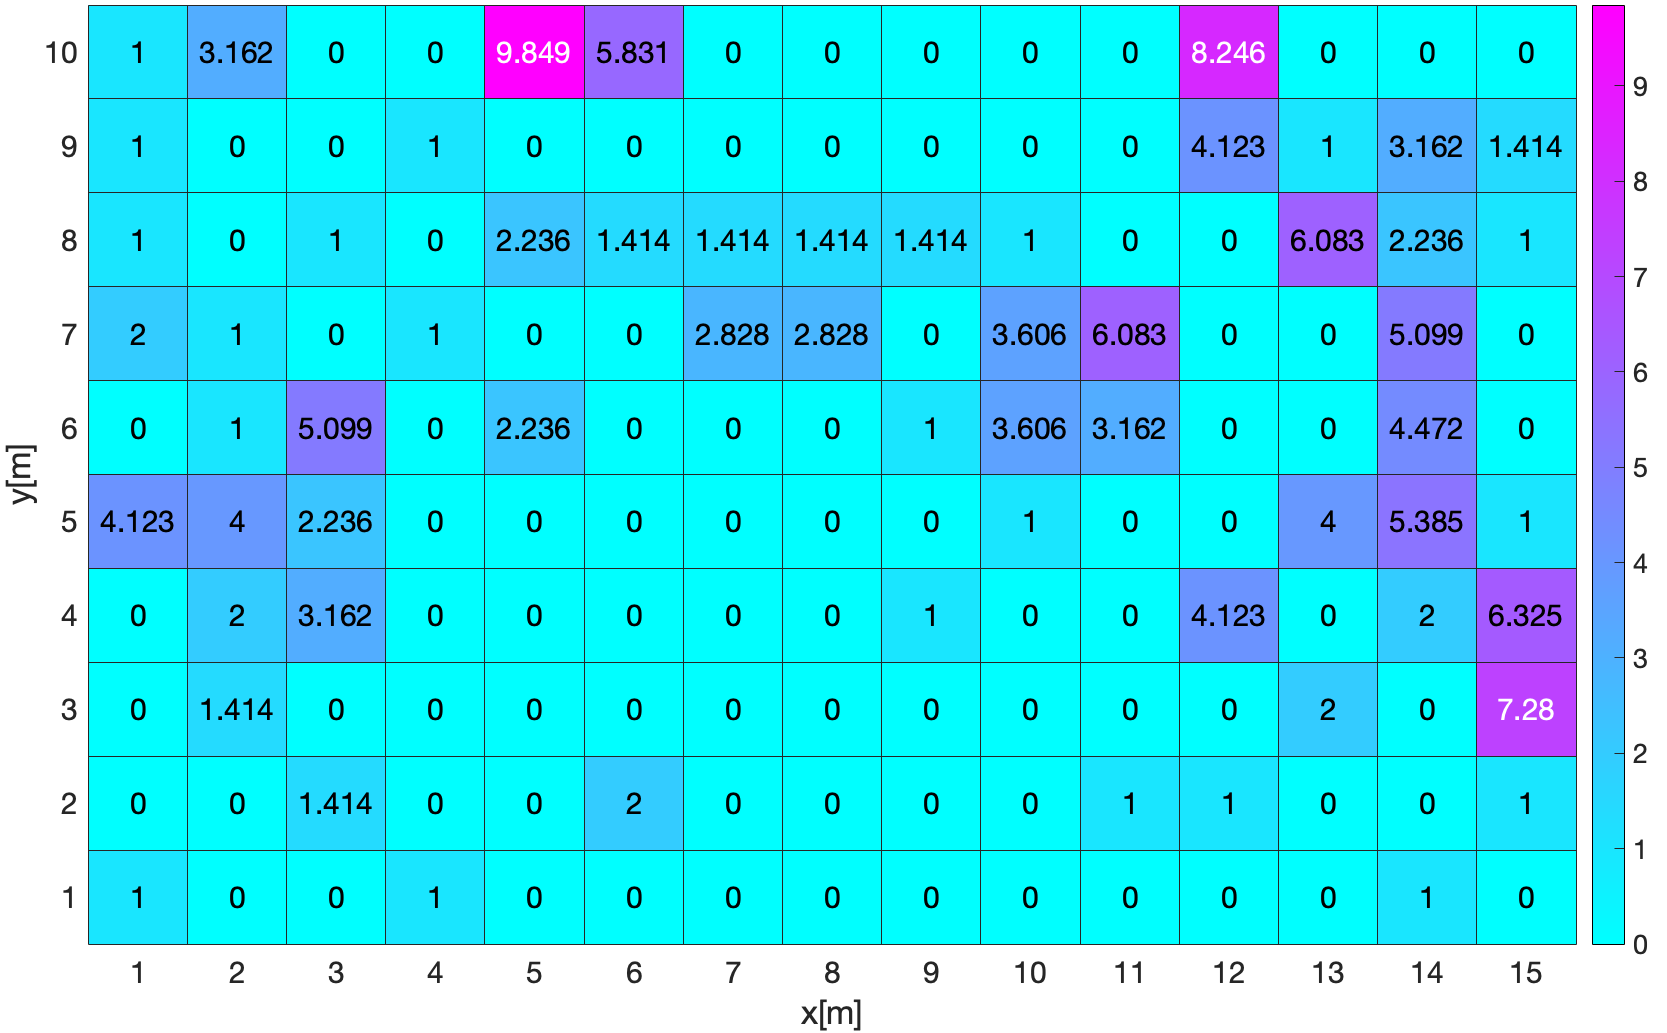
\includegraphics[width=\linewidth]{Images/no_more_name_idea.png}
\caption{Distance [m] between the tag location and its estimation using the \gls{sla}. Anchor being located in (3, 1). \label{fig:pos_ant_empty_non_sym}}
\end{figure}

We can observe that some locations have an error relatively big in comparison to the size of the room. For example, at the point (15, 3), the error made is about 7.3 m. To analyse the source of the error, a map of the \gls{mse} computed between the realistic \gls{cir} and the theoretical \gls{cir} computed at each location is drawn on Fig. \ref{fig:mse_analysis}. We can see that the best \gls{mse} is located at (13, 10) instead of the (15, 3) expected which corresponds to the distance error of 7.3 m.

\begin{figure}[H]
\centering
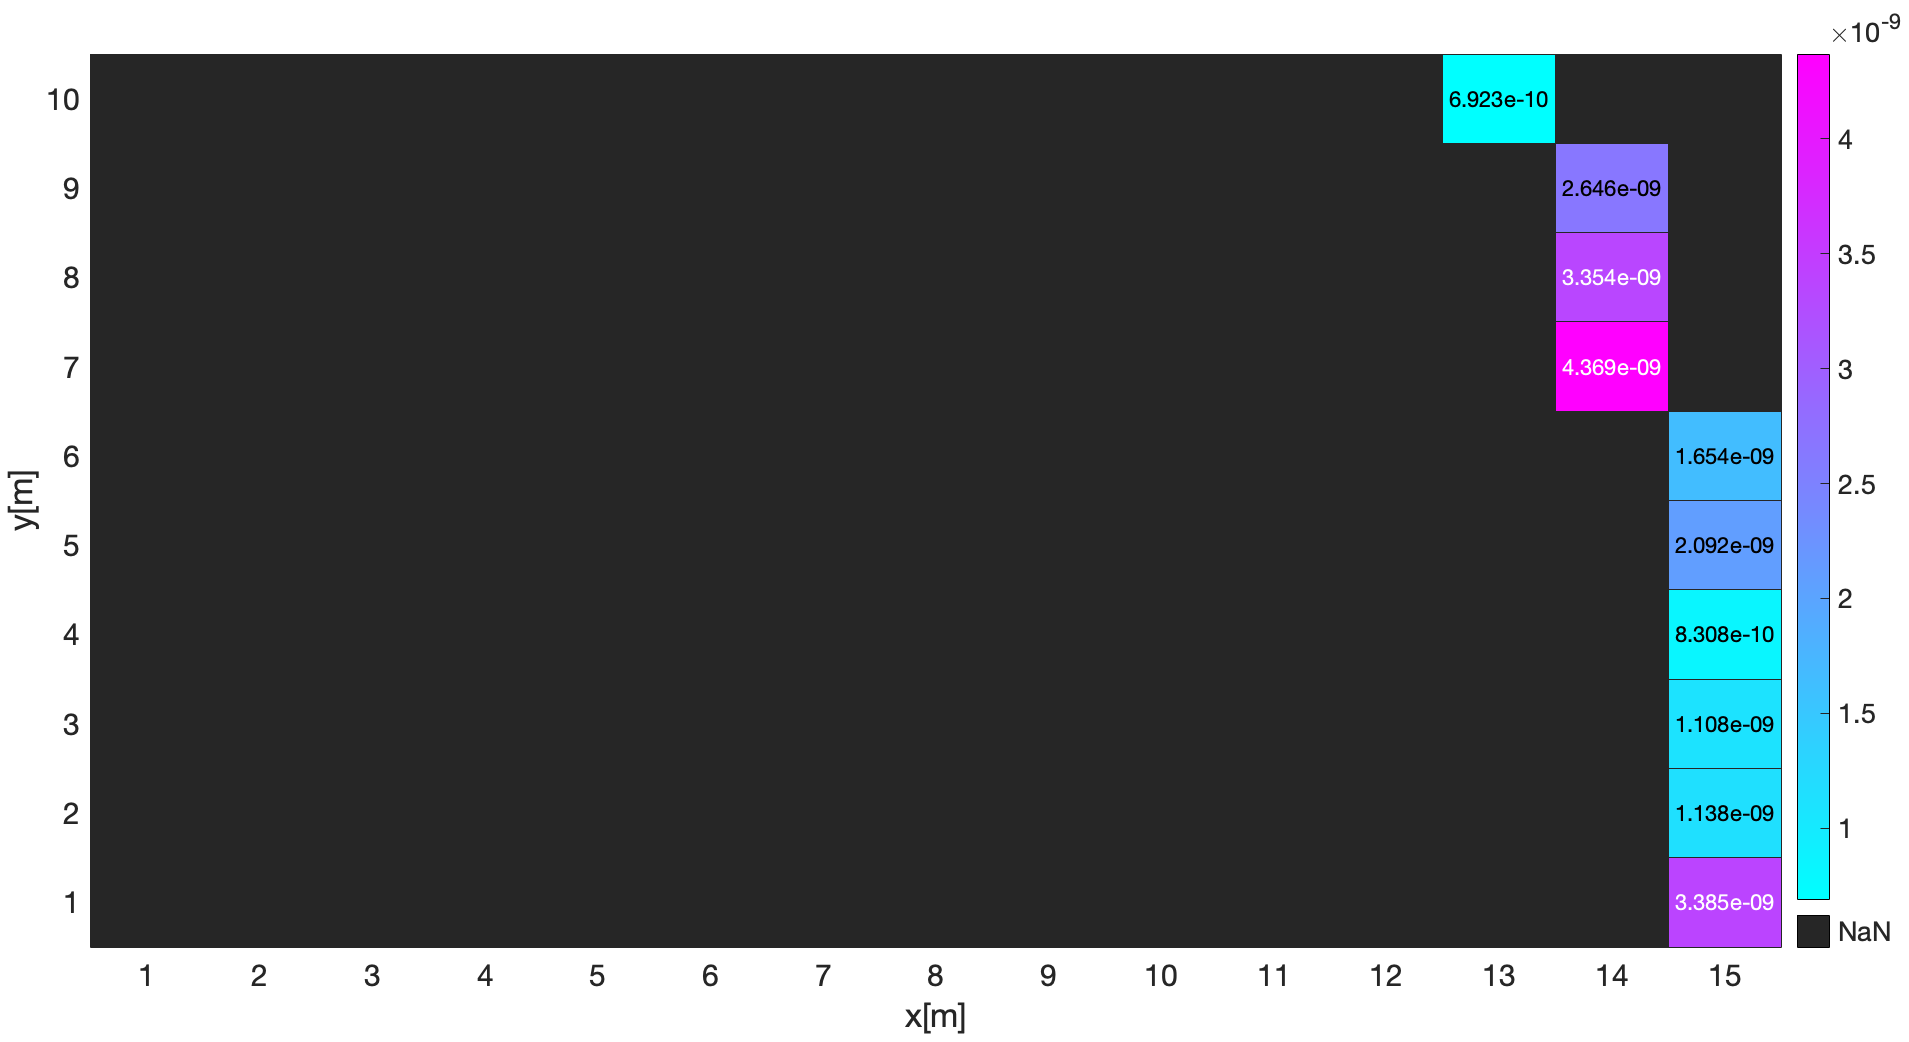
\includegraphics[width=\linewidth]{Images/no_name_1.png}
\caption{CIR BLABLABLA). \label{fig:mse_analysis}}
\end{figure}

It can be interesting to compare the full \gls{cir} instead of only comparing the peaks. This is what is shown on Fig. \ref{fig:cir_compa}, the top \gls{cir} being the realistic, the middle corresponding to the \gls{cir} originating from the tag exact location while the bottom \gls{cir} corresponds to the one at coordinates (13, 10), where the best \gls{mse} can be found.

\begin{figure}[H]
\centering
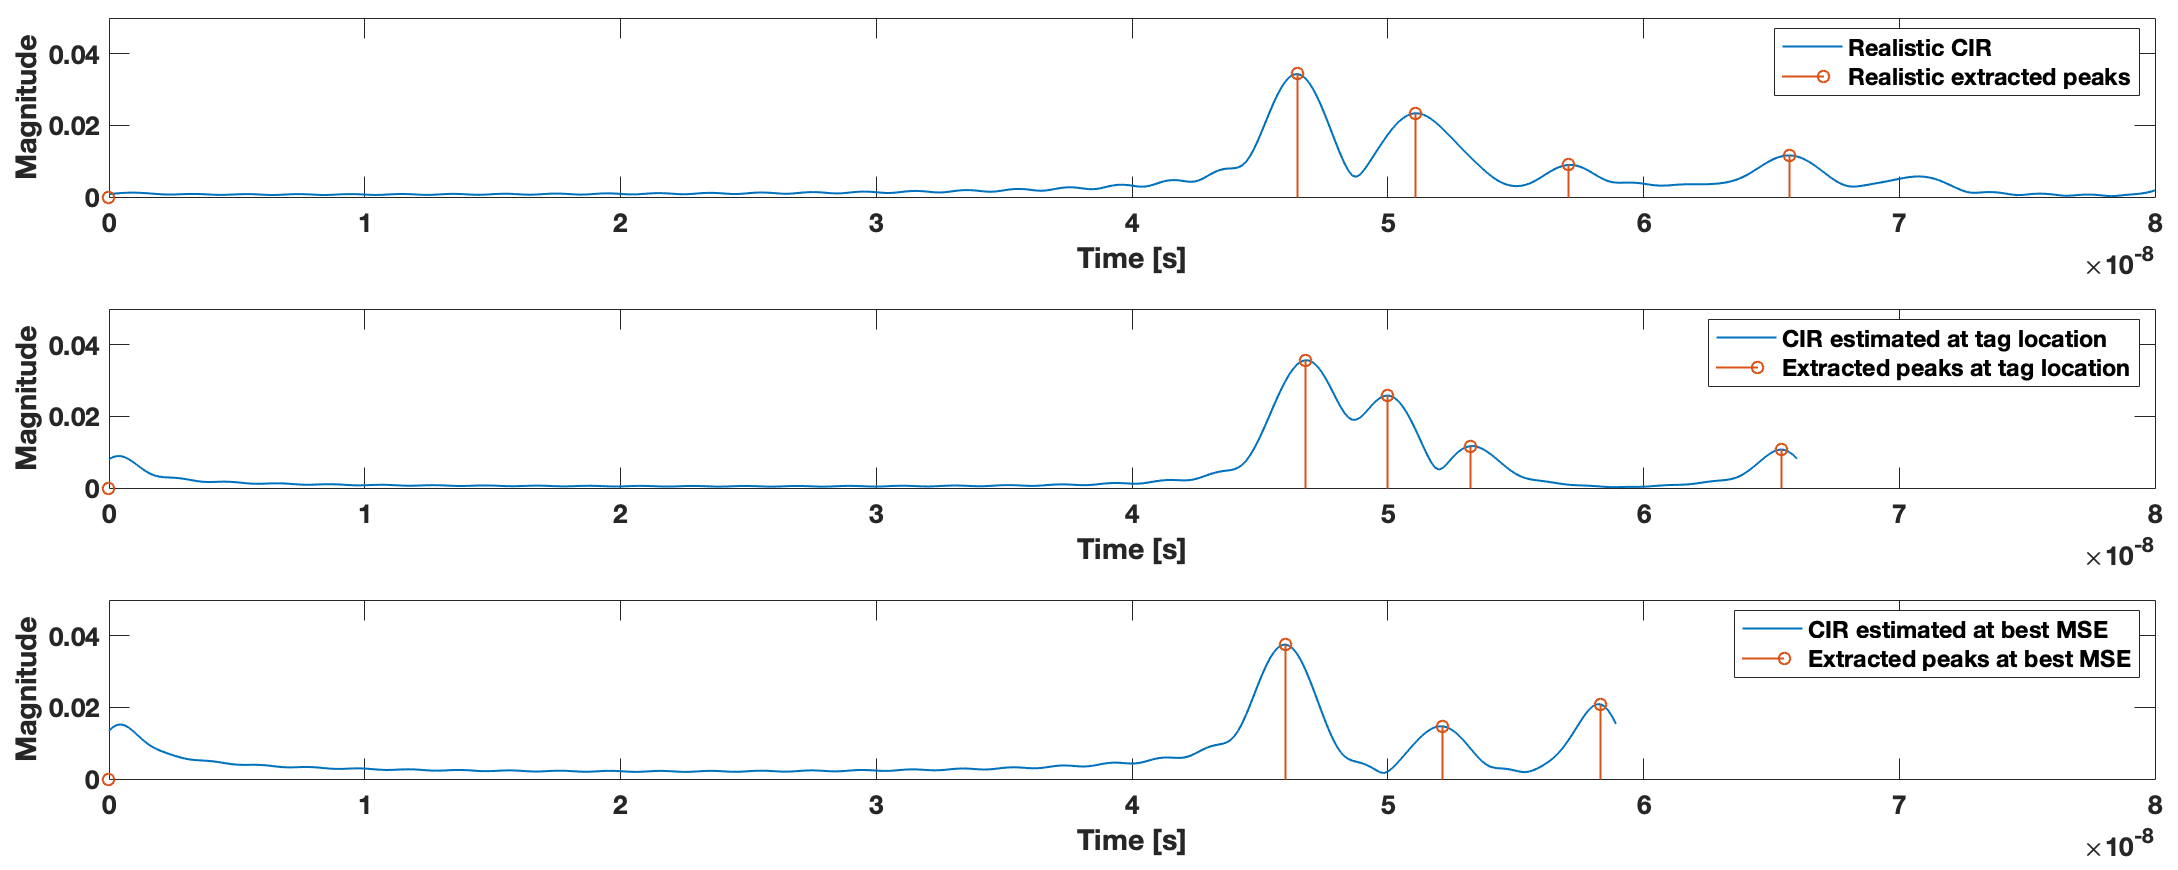
\includegraphics[width=\linewidth]{Images/no_name_2.png}
\caption{CIR BLABLABLA). \label{fig:cir_compa}}
\end{figure}

Several observations can be made. First, it can be seen that the form of the middle \gls{cir} does not fully correspond to the top \gls{cir}. Those difference in the form can mostly be attributed to the multiple reflections that take place in the top \gls{cir}. From that moment, if the two \gls{cir} are too different, the \gls{sla} will have some difficulties to compare them and find a theoretical \gls{cir} that really matches the realistic.
\vspace{2mm}

Concerning the bottom \gls{cir}, this one have been chosen by the algorithm by default. Since no \gls{cir} stood out, meaning that the extracting peaks from the theoretical \gls{cir} did not fully correspond to the realistic as in \ref{fig:soft_simu}, the less worst in term of \gls{mse} was chosen.
\vspace{2mm}

\subsubsection{Soft part of the algorithm}

This algorithm is call soft because of the \gls{mse} map produced as in Fig. \ref{fig:mse_analysis}. Instead of returning the location where the \gls{mse} has the lower value, we could evaluate the area where the \gls{mse} is the minimal in average.
\vspace{2mm}

In this example, while the location (13, 10) clearly has the lowest \gls{mse}, (15, 4) also has a \gls{mse} of magnitude $10^{-8}$. It also appears that (15, 4) is surrounded by some relatively low \gls{mse} values. We could therefore use this algorithm not solely based on the lowest \gls{mse} computed but also based on the probability to be in a specific area filled with low \gls{mse} values.
\vspace{2mm}

This solution is not an optimal one and may not solve every possible location. For example, Fig. \ref{fig:again_an_image} shows the \gls{mse} map for the tag location (14, 6). The estimated location being (15, 2) would not slightly change using this probability map.

\begin{figure}[H]
\centering
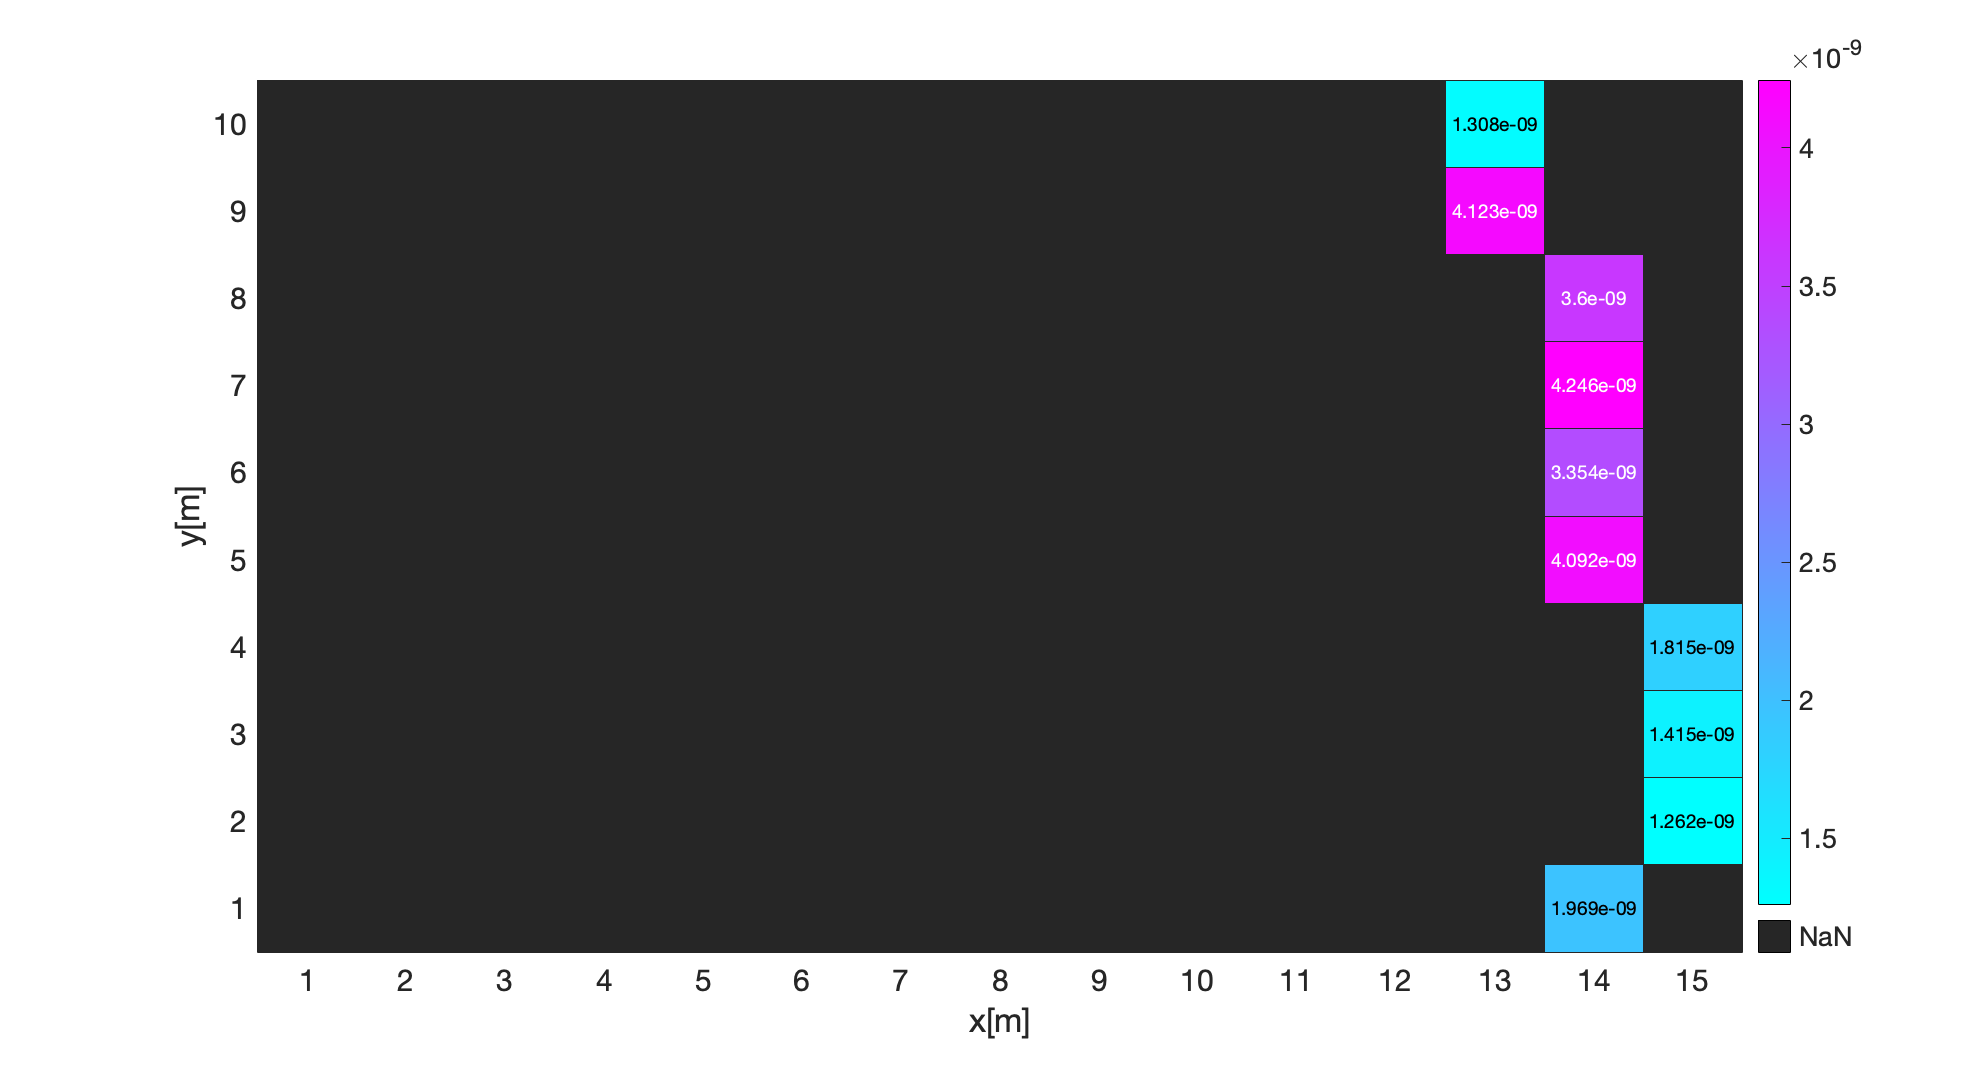
\includegraphics[width=.9\linewidth]{Images/image_XXX.png}
\caption{Find name \label{fig:again_an_image}}
\end{figure}

In definitive, in a perfect non cluttered room, the \gls{sla} does not reach a perfect score on the localization in comparison with the three anchor model in \cite{hannotier2019indoor}. It may be possible to improve the localisation and give a confidence interval based on a \gls{mse} map as in Fig. \ref{fig:cir_compa}.

\subsection{Soft localization in a cluttered room}

The simulations of this section have been done for a room of the same dimension as section \ref{soft_empty_room} filled with furniture. Four different consoles of various sizes are placed against each wall of the room. This will results in are realistic \gls{cir} being more complex because of the various reflections taking place on the walls and the furniture. The used room can be seen in Fig. \ref{fig:room_cluttered}. The furniture considered in this section are those in brown.

\begin{figure}
\centering
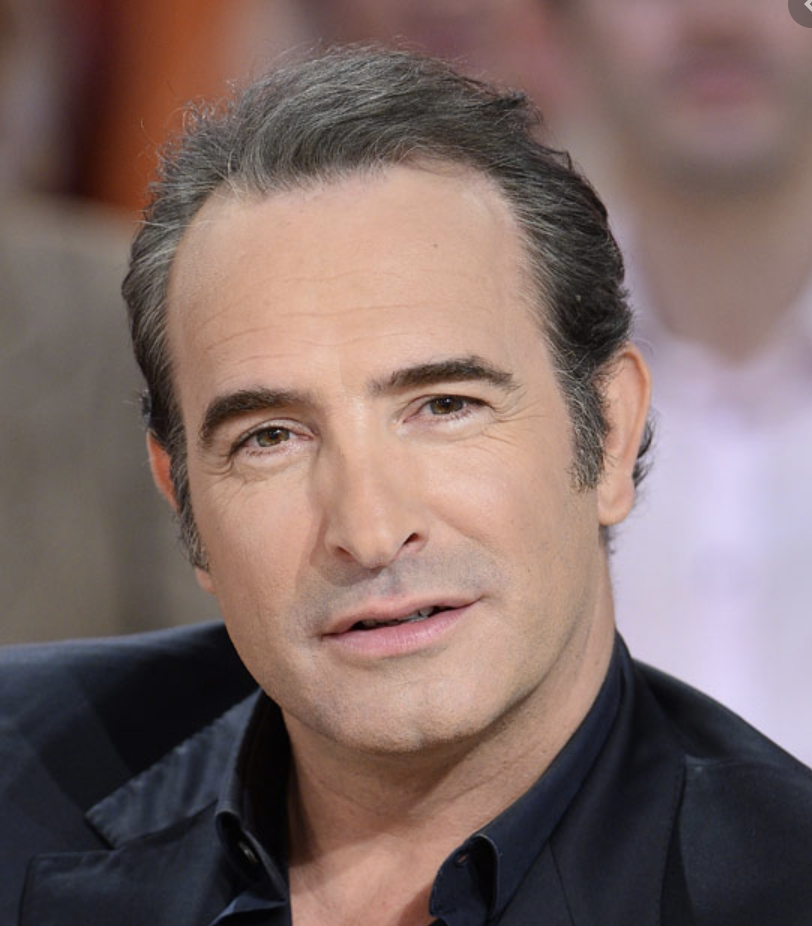
\includegraphics[width=.2\linewidth]{Images/Temporary_pic.png}
\caption{Cluttered room \label{fig:room_cluttered}}
\end{figure}




\section{Hard Simulation}


